\section{UAV dynamics}
\label{chap:uav_dynamics}

Modeling a system dynamics has always been a great part of a control design process. One with a good understanding of a system's behavior can design a well suited controller using various approaches taught in the field of control theory. Such controller can reflect known characteristics of the system and can appropriately react to evolution of system states. There are two fundamental approaches to the system modeling. One is based on the knowledge about the physics involved in the system. This knowledge can be used to derive a mathematical model using known principles, e.g. Hamiltonian mechanics. Control design a well known system is usually called WhiteBox, or GreyBox, depending on how much of the physical process we are able to describe. On the other hand, when the system is unknown, one can create a mathematical model which sufficiently represents observed behavior of the system. Such method is usually called BlackBox.

When modeling a classical helicopter, a complex model including phenomena as aerodynamics and rotor-blade flapping could be made. In many cases~\citep{alexis2014robust}\citep{mahony2012multirotor}, dynamics of a multirotor MAV can be simplified to a single rigid-body description, mostly because of smaller fixed-pitch propellers. Further due to existence of well designed and tested platforms such as Pixhawk~\citep{pixhawk} or Ardupilot~\citep{ardupilot} the vehicle can be modeled with the inner feedback loop closed. By doing that, considering a fixed-pitch quadrotor, we move from a system actuated by thrust of its four propellers to a system, where the inputs are the desired pitch ($\theta_D$), roll ($\psi_D$), yaw rate ($\dot{\phi}_D$) and collective thrust ($U_D$). It is assumed that such system can be treated as a decoupled system~\citep{mahony2012multirotor}. Some assumptions and simplifications are made in the following chapter thus the field of modeling is the GreyBox.

%Following chapter shows how the UAV's dynamics can me modeled based on the Newton's 2nd law of motion

\begin{figure}[!h]
\centering
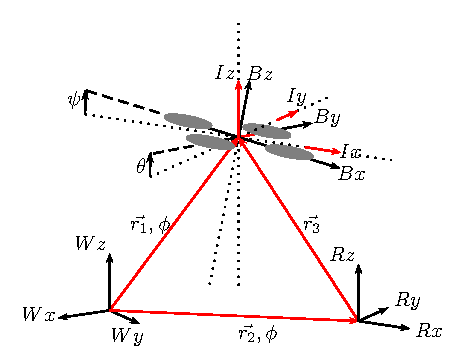
\includegraphics[width=0.7\textwidth]{fig/coordinate_system.pdf}
\caption{UAV and its coordinate systems}
\label{fig:coordinate_system}
\end{figure}

\subsection{Attitude dynamics}

There are several coordinate systems in which states of the UAV~(Figure~\ref{fig:coordinate_system}) are expressed. There is a world coordinate system \textit{W} with a fixed position in the world. Then there is a rotating world coordinate system \textit{R}. It is rotated from $W$ by the angle $\phi$. Following is an inertial frame \textit{I} in which the attitude angles $\theta$ and $\psi$ are measured. It is translated into the geometric center of the UAV. At last there is a body frame \textit{B} which axis are aligned with the mechanical frame of the UAV.

Assuming a complete decoupling of the system, the lateral dynamics can be expressed by following equations:

\begin{equation}
\begin{split}
\ddot{x}^W &= \frac{U}{m}\left(\sin\psi\cos\phi + \sin\theta\sin\phi\right),\\
\ddot{y}^W &= \frac{U}{m}\left(\sin\theta\cos\phi + \sin\psi\sin\phi\right),\\
\end{split}
\end{equation}

where $U$ is a the total thrust force action on a center of gravity\footnote{in a direction of the $B_z$ axis} and $m$ is the mass of the UAV. It is assumed that desired operating point is a hovering state, where $U$, $m$ are constant and $\theta$, $\psi$ are around zero. We can then simplify the equations into the following form:

\begin{equation}
\begin{split}
\ddot{x}^R &= K_1\sin \phi,\\
\ddot{y}^R &= K_1\sin \theta.\\
\end{split}
\label{eq:attitude_first_lin}
\end{equation}

Since our system is not placed under a global localization system and it relies completely on a dead-reckoning in terms of stabilizing the yaw motion\footnote{The yaw angle $\phi$ is stabilized by a feedback loop implemented on a stabilization board using onboard IMU}, all positions and its derivatives in following equations are expressed in system $R$. Furthermore assuming a small input actions during hovering around the operating point, these forms can be linearized. It is done by approximating it by first two terms of the Taylor series.

\begin{equation}
\begin{split}
\ddot{x} &= K_1 \phi,\\
\ddot{y} &= K_1 \theta.\\
\end{split}
\end{equation}

\subsection{Altitude dynamics}

The altitude dynamics is described by following equation

\begin{equation}
\begin{split}
\ddot{z} &= \frac{U}{m}\cos\theta\cos\psi - g^W,
\end{split}
\end{equation}

where $g^W$ is a gravitational acceleration. This system is also non-linear, but we need to be more cautious with a potential linearization in this case. If we try to build an altitude controller which is supposed to work not only around a hovering point, but also during take-off and landing. Unlike in~(\ref{eq:attitude_first_lin}), the force $U$ should not be treated as constant. The pull force of a propeller can be simplified to a quadratic function of its angular speed [\strong{REFERENCE}], which is one of the controlled inputs.

\subsection{Dynamics of the integrated stabilization}

Current UAVs are usually equipped with an attitude stabilization system. When building a custom multirotor, such system can be a cheap and affordable item on a list. If properly tuned and the feedback loop is closed it transforms the system to be controlled by $\theta_D$, $\psi_D$, $U_D$, $\dot{\phi_D}$, instead of desired thrust of each motor. For purposes of this thesis, all four model systems are modeled using first order transfer function (\ref{eq:first_order_stab}). Furthermore it is shown (chapter~\ref{cap:system_identification}) that these models are satisfactory and can be well fitted on a measured data. It is assumed that there is not present any altitude feedback loop\footnote{which would require e.g. barometer, GPS, ...}. In that case, the first order system would encapsulate also one of system's integrators ($\ddot{z} \rightarrow \dot{z}$) considering an altitude speed controller which is common in some systems \citep{pixhawk}\cite{ardupilot}.

\begin{equation}
\begin{split}
\frac{\mathcal{L}\left\lbrace U \right\rbrace}{\mathcal{L}\left\lbrace U_D \right\rbrace} = \frac{\mathcal{L}\left\lbrace \theta \right\rbrace}{\mathcal{L}\left\lbrace \theta_D \right\rbrace} = \frac{\mathcal{L}\left\lbrace \psi \right\rbrace}{\mathcal{L}\left\lbrace \psi_D \right\rbrace} = \frac{\mathcal{L}\left\lbrace \dot{\phi} \right\rbrace}{\mathcal{L}\left\lbrace \dot{\phi}_D \right\rbrace} = \frac{1}{\tau s + 1}\\
\end{split}
\label{eq:first_order_stab}
\end{equation}

\subsection{State space representation}

For the purpose of this thesis the discrete formulation of the dynamical system will be used. It allows to formulate proper filtration method and the MPC controller itself. Since now, all differential equations and state space formulation are written in a discrete form with a constant sampling rate $1/\Delta t$. Following form describes a discrete time-invariant system with a main matrix $\mathbf{A}$, and input matrix $\mathbf{B}$

\begin{equation}
\mathbf{q}_{t+1} = \mathbf{A}\mathbf{q}_{t}+ \mathbf{B}\mathbf{u}_{t},
\end{equation}

where $\mathbf{x}_{t}$ is the state vector in the sample time $t$. Following matrices describe the pitch and roll systems given the state vectors $\mathbf{q}_{x} = \left(x, \dot{x}, \ddot{x}\right)$, $\mathbf{q}_{y} = \left(y, \dot{y}, \ddot{y}\right)$ and inputs $\mathbf{u}_x = \theta_D$, $\mathbf{u}_y = \psi_D$

\begin{equation}
\begin{split}
\mathbf{A}_{x, y} = \begin{bmatrix}
1 & \Delta t & 0 \\
0 & 1 & \Delta t \\
0 & 0 & P_1
\end{bmatrix}, \mathbf{B}_{x, y} = \begin{bmatrix}
0\\
0\\
P_2
\end{bmatrix},
\end{split}
\end{equation}

where $\Delta t$ is the sampling period, $P_1$ and $P_2$ are parameters of the first order transfer from a desired to the actual angle of attitude. This system description is an LTI system and can be directly used for state estimation (using e.g. Kalman filter) or for a MPC controller. For purpose of modeling altitude dynamics including Earth's gravitational pull, we can add an additional input to the system which will act as an constant source of acceleration. In the following case the 2nd input's value is always equal to $1$. Eq. (\ref{eq:altitude_LTI}) shows the discrete altitude LTI system for state vector $\mathbf{q}_{z} = \left(z, \dot{z}, \ddot{z}\right)$ and input $\mathbf{u}_z = \dot{U}_D$ linearized around a hovering point

\begin{equation}
\begin{split}
\mathbf{A}_{z} = \begin{bmatrix}
1 & \Delta t & 0 & 0\\
0 & 1 & \Delta t & 0\\
0 & 0 & 0 & 1 \\
0 & 0 & 0 & P_3
\end{bmatrix}, \mathbf{B}_{z} = \begin{bmatrix}
0 & 0\\
0 & 0\\
0 & -g\\
P_4 & 0
\end{bmatrix},
\end{split}
\label{eq:altitude_LTI}
\end{equation}

where $g \approx 9.8 ms^{-2}$ is a gravitational acceleration, $P_3$ and $P_4$ are parameters of the first order system $U_D \rightarrow \ddot{z}$. The last system represents the yaw dynamics of the UAV for state vector $\mathbf{q}_{\phi} = \left(\phi, \dot{\phi}\right)$ and input $\mathbf{u}_\phi = \dot{\phi}_D$

\begin{equation}
\begin{split}
\mathbf{A}_{\phi} = \begin{bmatrix}
1 & \Delta t\\
0 & P_5 \\
\end{bmatrix}, \mathbf{B}_{\phi} = \begin{bmatrix}
0\\
P_6
\end{bmatrix},
\end{split}
\end{equation}

where $P_5$ and $P_6$ are parameters of the system $\dot{\phi}_D \rightarrow \dot{\phi}$.